\newcommand{\blockdiagram}[4]{
	\begin{tikzpicture}[font=\sffamily,>=triangle 45]
         \node [circuit] (item) {};
		
		\matrix[
		matrix of nodes,
		left= of item,
		row sep=\myheight/15,
		nodes={anchor=east}
		] (rightmatr) {
			#3
			\\
		};
		\matrix[
		matrix of nodes,
		right= of item,
		row sep=\myheight/15,
		nodes={anchor=west}
		] (leftmatr) {
			#4
			\\
		};
	
		\foreach \i in {1,...,#1}
			\draw [->] (rightmatr-\i-1) -- (rightmatr-\i-1 -| item.west);
		\foreach \i in {1,...,#2}
			\draw [<-] (leftmatr-\i-1) -- (leftmatr-\i-1 -| item.east);
	\end{tikzpicture}
}


\chapter{Architettura ed implementazione}

L'architettura da sintetizzare su FPGA è stata sviluppata utilizzando il linguaggio VHDL, facendo
ampiamente uso di molte funzionalità della versione VHDL-2008.
Il progetto è stato sintetizzato usando il software Vivado 2018.2 della Xilinx e simulato usando il compilatore/simulatore open-source GHDL.

Dal punto di vista architetturale si può considerare il progetto come composto da due macro-blocchi indipendenti: uno che si occupa di gestire i segnali MIDI dati in input al sintetizzatore, e uno che si occupa di generare il segnale audio in uscita.

Le due componenti sono implementate in logica sincrona e sono collegate da una lookup table che memorizza le note attive. Alla ricezione di un evento MIDI \textit{note on} il bit corrispondente alla nota nella LUT viene portato al valore logico alto, e al seguente istante di campionamento la componente che genera il segnale di output userà questo valore per determinare se suonare o meno la nota.

\section{Scelta dei parametri di progetto}
Mentre la frequenza di clock $f_{clk} = \SI{100}{\mega\hertz}$ e 
la frequenza di campionamento minima $f_{s,min} = 2 \cdot \SI{21000}{\hertz}$
sono date, non sono note a priori i seguenti parametri:
\begin{itemize}
    \item \textbf{\code{b}}: Numero di bit usati per quantizzare la forma d'onda
    \item \textbf{\code{N}}: Numero di bit usati per il registro di fase nel phase accumulator
    \item \textbf{\code{M}}: Numero di bit presi tra i primi bit del registro di fase e usati per indirizzare i campioni
\end{itemize}

Utilizzando i vincoli imposti dalla conversione D/A in PWM, si 
ottiene il numero massimo di bit del quantizzatore imponendo che

\[
\code{b} < \lceil \log_{2}{\frac{f_{clk}}{f_{s,min}}} \rceil = 12
\]

Conviene quindi massimizzare \code{b} per avere una minore errore di quantizzazione,
e allo stesso tempo massimizzare il più possibile $f_s$, scegliendola per comodità
come sottomutiplo della frequenza di clock.
Si ottiene così $\code{b} = 11$ e $f_s = \SI{48828}{\hertz}$

Nella seguente tabella sono riportati i valori dei parametri e, in aggiunta, i relativi
nomi all'interno del progetto VHDL.

\begin{tabular}{| c | c | m{10em} | l | }
 \hline
 \textbf{Parametro} & \textbf{Valore} & \textbf{Descrizione} & \textbf{VHDL constant}\\
 \hline
 $f_{clk}$  & \SI{100}{\mega \hertz} & frequenza di clock del FPGA  & \code{clock\_frequency}\\
 \hline
 $f_s$ &  \SI{48828}{\hertz} & frequenza di campionamento & \code{sampling\_frequency}\\
 \hline
 \code{b} & 11 & numero di bit dei campioni & \code{sample\_bits}\\
 \hline
 \code{N} & 32 & numero di bit del registro di fase e della frequency tuning word & \code{phase\_bits}\\
 \hline
 \code{M} & 13  & numero di bit degli indirizzi dei campioni & \code{address\_bits}\\
 \hline
\end{tabular}

\section{Componenti fondamentali}
I seguenti blocchi fondamentali corrispondono in VHDL al costrutto di \textit{entity} e veranno analizzati dettagliatamente in seguito:

TODO: aggiungere contatore e low\_to\_high\_detector
\begin{itemize}
	\item \hyperref[sec:uart]{uart} Si occupa della ricezione seriale a 31250 baud secondo le specifiche MIDI
	\item \hyperref[sec:mididec]{midi\_decoder}  State machine che codifica i byte ricevuti dal blocco uart in eventi MIDI; gestisce solamente gli eventi note on/off
	mentre scarta tutti gli altri eventi MIDI.
	\item \hyperref[sec:noteslut]{active\_notes\_lut} Tabella di lookup contenente 128 valori booleani che indicano l'attivazione di una nota
	\item \hyperref[sec:phaseaccumulator]{phase\_accumulator} Opera l'accumulazione di fase per la DDS
	\item \hyperref[sec:pwmencoder]{pwm\_encoder} Genere la modulazione PWM corrispondente in uscita
	a partire da un campione fornito in entrata
	\item \hyperref[sec:rom]{rom} Package generico che rappresenta una read-only memory.
	\item \hyperref[sec:synthengine]{synth\_engine} Cuore del sintetizzatore, provvede alla DDS a partire dai valori presenti in active\_notes\_lut, alla phase-to-amplitude conversion attraverso una ROM e al mixing.
	\item synth\_top Entità top del progetto, cioè che contiene tutte le altre entity e le istanzia nel modo corretto, impostando le frequenze di lavoro dei componenti.
\end{itemize}

\section{Blocco UART}
\label{sec:uart}

%\begin{lumos}
%	\luminput{
%		i\_clock \\
%		i\_serial\_input \\
%	}
%	\lumoutput{
%		o\_data\\
%		o\_data\_available
%	}
%\end{lumos}

\begin{center}
	\blockdiagram{2}{2}{
		i\_clock \\ i\_serial\_input
	}{
	    o\_data \\ o\_data\_available
    }
\end{center}

Il blocco uart è composto da una finite state machine (fsm) e uno shift register da 9 bit, contenente inizialmente i valori '0' tranne per il bit più significativo che è posto a '1' e funge da sentinella. La lettura della linea dati avviene periodicamente alla frequenza $f = \frac{1}{T_{bit}} = 31250 \si{Hz}$; alla ricezione dello start bit, la fsm entra nello stato di ricezione e si fa avanzare lo shift register leggendo il valore presente sulla linea nel bit più significativo, facendo contemporaneamente slittare gli altri verso destra.
A lettura ultimata, lo shift register sarà avanzato di 8 posizioni e il bit meno significativo dello shift register contiene il bit sentinella; con questo si indica la fine della trasmissione.

\section{MIDI decoder}
\label{sec:mididec}

\begin{center}
	\blockdiagram{3}{2}{
		i\_clock \\
		i\_enable \\
		i\_data \\
	}{
	    o\_message \\
	    o\_message\_available
    }
\end{center}
Il decoder MIDI si occupa di leggere i byte provenienti dal convertitore seriale/parallelo e di convertirli in messaggi MIDI.
In realtà il componente è molto semplificato in quanto interpreta solo i messaggi di note on e note off, mentre scarta ogni altro messaggio MIDI.
Il blocco è implementato attraverso una fsm; quando l'input \code{i\_enable} viene mantenuto alto per un ciclo di clock, la state machine avanza leggendo il byte \code{i\_data} in input.
Quando il messaggio è stato completamente decodificato, l'output \code{o\_message\_available} assume un valore logico alto e il messaggio MIDI è disponibile in uscita al blocco.

\section{Active Notes LUT}
\label{sec:noteslut}

\begin{center}
	\blockdiagram{3}{1}{
		i\_clock \\
		i\_enable \\
		i\_message \\
	}{
		o\_active\_notes\_reg
	}
\end{center}
Quando il segnale \code{i\_enable} è alto per un ciclo di clock, il valore del messaggio midi in input viene letto e il registro \code{o\_active\_notes\_reg} viene modificato in modo che il bit in posizione corrispondente alla nota sia 1 o 0 a seconda che il messaggio sia note on oppure note off.

\section{Accumulatore di Fase}
\label{sec:phaseaccumulator}

\begin{center}
	\blockdiagram{3}{1}{
		i\_clock \\
		i\_rst\_sync \\
		i\_ftw \\
	}{
		o\_phase\_reg
	}
\end{center}
Parlare dei parametri generici
L'accumulatore di fase è un registro che viene incrementato ad ogni ciclo di clock del valore presente in ingresso alla porta \code{i\_ftw}.
È possibile il reset sincrono del registro impostando al valore logico alto il segnale \code{i\_rst\_sync}

\section{PWM Encoder}
\label{sec:pwmencoder}

\begin{center}
	\blockdiagram{2}{1}{
		i\_clock \\
		i\_sample
	}{
		o\_pwm\_signal
	}
\end{center}
L'encoder PWM si occupa di leggere il campione presente alla porta i\_sample alla frequenza $f_s$ di campionamento
Scrivere considerazioni sul range del segnale di uscita, codifica, aritmetica con segno.
Scrivere riguardo ad alta impedenza
\begin{figure}
	\centering
	\def\svgwidth{\columnwidth}
	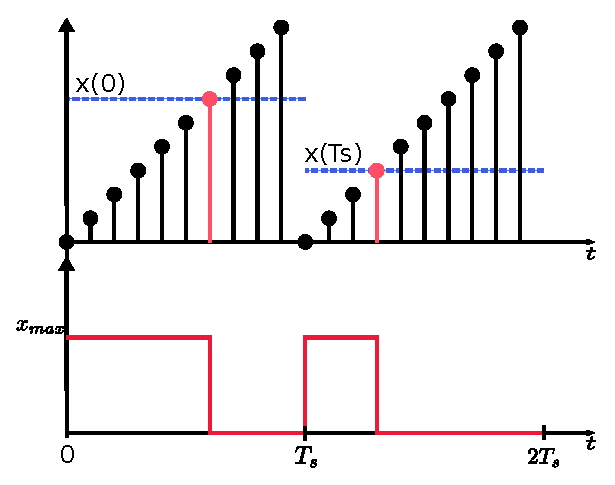
\includegraphics[width=0.7\columnwidth]{TeX_files/pwm_ramp.eps}
	\caption{Esempio di PWM: nel grafico sopra è riportato il valore del campione $x(kT_s)$ (tratteggio blu), che viene comparato al contatore.
	Quando il contatore supera il valore di $x(kT_s)$, \code{o\_pwm\_signal} passa da $x_{max}$ a $0$. }
\end{figure}

\section{Componente ROM}
\label{sec:rom}
Le ftw e la forma d'onda da riprodurre vengono generate attraverso due
script python e salvate in un file.
Il package generico rom permettere al progetto di avere queste informazioni in fase di sintesi: si specificano i tre parametri \code{word\_bits}, che indica il numero di bit per parola nella memoria, \code{address\_bits}, che indica il numero di bit necessari a indirizzare una parola, e \code{rom\_filename}, che specifica il file testuale da leggere contenente le parole della rom.
Il file deve essere formattato nel seguente modo: ci sono tante righe quanti sono gli indirizzi della memoria, ogni riga è una stringa binaria
di lunghezza fissa e rappresenta la parola memorizzata.
Gli indirizzi partono da 0 (prima riga) e aumentano di un unità ad ogni riga.
È possibile leggere dalla ROM usando la funzione \code{read\_at}, specificando come argomento l'indirizzo desiderato.

\begin{minted}{VHDL}
package rom is
  generic (
    word_bits: positive;
    address_bits: positive;
    rom_filename: string
  );
  subtype word_type is std_logic_vector(word_bits-1 downto 0);
  impure function read_at(
     address: in integer range 0 to 2**address_bits-1
  ) return word_type;
end package rom;
\end{minted}

\section{Synth Engine}
\label{sec:synthengine}

\begin{center}
	\blockdiagram{2}{2}{
		i\_clock \\
		i\_active\_notes
	}{
		o\_sample \\
		o\_sample\_ready
	}
\end{center}


Il componente principale del sintetizzatore ha accesso alla LUT contenenti le note attive e genera ad ogni periodo di campionamento
un campione del segnale.

Attraverso il package \hyperref[sec:rom]{rom} vengono rese disponibili a questo componente la forma d'onda campionata e le frequency
tuning word corrispondenti ad ogni possibile nota suonata.
Attraverso il costrutto \code{for .. generate} vengono generati 128 accumulatori di fase indipendenti. Ad ognuno di questi viene accoppiata
una entity che ne esegue il reset quando una nota passa dal valore logico basso a quello alto nella LUT.

\begin{minted}{VHDL}
oscillators:
for i in 0 to MAX_MIDI_NOTE_NUMBER generate
    signal ftw: std_logic_vector(phase_bits-1 downto 0);
    signal reset_signal: std_logic := '0';
begin
    ftw <= phase_rom.read_at(i);
    reset_generator: entity work.low_to_high_detector
    port map (
        i_clock => i_clock,
        i_signal => i_active_notes(i),
        o_detected => reset_signal
    );
    accumulator: entity work.phase_accumulator
    generic map (
        clock_frequency => clock_frequency,
        phase_bits => phase_bits
    )
    port map (
        i_clock => i_clock,
        i_rst_sync => reset_signal,
        i_ftw => ftw,
        o_phase_reg => phase_vec(i)
    );
end generate oscillators;
\end{minted}

Il campione viene fornito alla porta \code{o\_sample} e viene generato attraverso un processo di mixing.
Il mixing consiste nel seguente processo, ripetuto per ogni valore della LUT delle note attive:
\begin{itemize}
    \item Se la nota è attiva, si carica il valore campionato della forma d'onda ad essa relativa:
          il valore campionato viene ottenuto dalla ROM dei campioni, usando come indice
          i primi \code{M} bit dell'accumulatore di fase: infatti questo è il
          \textbf{phase to amplitude converter} (PAC)
    \item Il valore del campione viene sommato su un registro inizialmente nullo
\end{itemize} 

Come verrà chiarito nella \cref{sec:timing_impl}
l'implementazione fa uso di una pipeline a due stadi:
il primo stadio della pipeline provvede alla PAC, mentre il secondo stadio
esegue parallelamente il mixing con il valore ottenuto dallo stadio
precedente.

Ogni avanzamento della pipeline viene eseguito in un ciclo di clock,
e in totale sono necessari 129 cicli di clock
(128 per ogni nota, più uno per caricare la pipeline) che vengono eseguiti
appena prima della fine del periodo di campionamento.
Questo avviene all'ultimo ciclo di clock della fase di produzione del
campione, in cui l'output \code{o\_sample\_ready} assume il valore
logico alto per indicare la presenza di un campione.
\begin{figure}
	\centering
	\def\svgwidth{\columnwidth}
	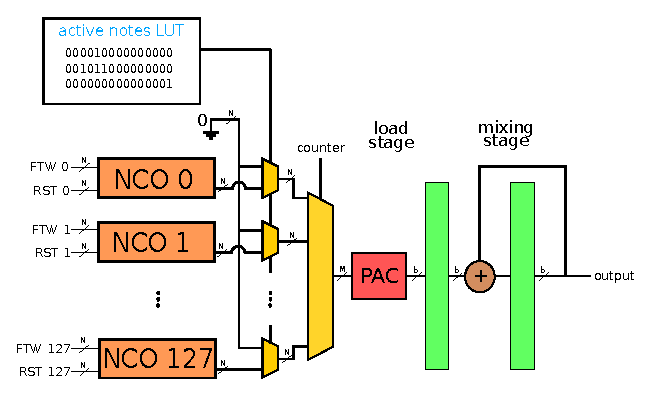
\includegraphics[width=\columnwidth]{TeX_files/synth_engine.eps}
	\caption{Architettura con pipeline a due stadi. Ogni multiplexer
	 in uscita ad un NCO controlla se la nota è attiva nella LUT; il
     multiplexer principale, comandato da un contatore, carica la pipeline
     con un nuovo campione. Seguono poi lo stadio di PAC (ossia il caricamento del campione dalla ROM) e il mixing.}
\end{figure}

TODO: commentare sul fatto che c'è ampio margine di tempo, magari calcolare
      (considerazione da spostare nella sezione successiva)

\section{Difficoltà di implementazione e vincoli temporali}
\label{sec:timing_impl}
Nel corso dello sviluppo del progetto una dei problemi più difficili da affrontare
è stato quello cdl rispetto dei vincoli temporali nell'implementazione dell'engine
del sintetizzatore.

Inizialmente questo era stato implementato come un componente asincrono, dotato di 
128 ingressi collegati alla LUT delle note attive, e 128 ingressi da \code{sample\_bits}
ciascuno collegati direttamente alla memoria dei campioni.
In totale il componente aveva quindi $128+128*11 = 1536$ bit in ingresso, senza contare
il sommatore e i multiplexer necessari alla selezione delle note.
Data la complessità del componente, questo veniva sintetizzato con una lunga catena
di sommatori a due ingressi collegati in cascata; tuttavia le catene di propagazione più lunghe
non rispettavano i vincoli temporali, avendo un WNS fino a ???

Si è quindi convertito il mixer in un componene sincrono, che sommasse ogni campione
ad un ciclo di clock; tuttavia anche in questo caso si ottenevano due path con WNS di ???

Una soluzione si sarebbe potuta ottenere dilatando il tempo tra due operazioni di somma
successive, impostando i parametri di progetti in modo da allentare i timing constraints
su queste path.
Un'altra soluzione simile sarebbe quella di usare un clock diverso per il processo di mixing.
Entrambe le soluzioni tuttavia richiedevano una conoscenza approfondita di Vivado,
e la seconda soluzione necessita della comunicazione tra componenti aventi 
clock diversi, detto \textit{clock domain crossing}, e molto complesso da
implementare.

Notando che la path che non rispettava i vincoli temporali attraversava
il sommatore, si è deciso di rendere l'operazione di caricamento del campione
e quella di somma distinte, formando così l'architettura a pipeline a due stadi descritta prima.

Così facendo il WNS diventa di $\SI{1.911}{\nano \second}$ e i vincoli temporali sono rispettati.
